\section{Binary Time Slicer}
\label{sec:timeslicer}

\subsection{Idea}
\begin{frame}{From the ISR experiments to a schedule}
  \begin{itemize}
    \item Chapter~\ref{sec:edsim}: work in an ISR is fine as long as it ends before the next interrupt; otherwise ticks are lost or the stack overflows.
    \item Typical application: several periodic jobs with different rates, e.g.\ read sensors every 1\,ms, control every 2\,ms, display every 4\,ms.
    \item \textbf{Time slicer}: one timer interrupt with period $T$ (the \emph{time slice}). Each tick calls \alert{exactly one} job function.
    \item \textbf{Binary} time slicer: the job is selected by the bit pattern of the tick counter, so every job gets a period $2^{k}\,T$.
  \end{itemize}
\end{frame}

\scriptonly{%
The experiments of Chapter~\ref{sec:edsim} showed what goes wrong when an interrupt service routine does more work than fits into its period. A time slicer turns the timer interrupt into a small, fixed schedule: the period of the timer is divided into slices of equal length $T$, and in every slice exactly one function, a \emph{job}, is executed. Because the jobs of one slice never meet the jobs of another, many problems of concurrent programs do not occur. The binary variant chooses the job from the binary representation of the tick counter, which needs neither tables of start times nor a scheduler, and still gives each job a fixed period.
}

\begin{frame}{The binary schedule}
  \begin{center}
  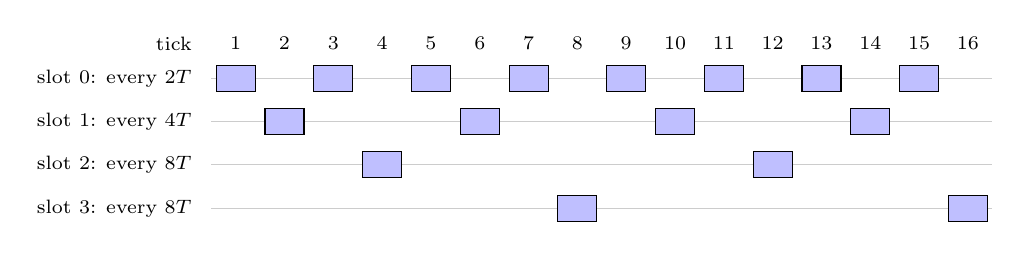
\begin{tikzpicture}[x=0.62cm,y=0.55cm,font=\scriptsize]
    \foreach \s/\lab in {0/{slot 0: every $2T$},1/{slot 1: every $4T$},2/{slot 2: every $8T$},3/{slot 3: every $8T$}}{
      \node[left] at (0.3,-\s) {\lab};
      \draw[gray!40] (0.5,-\s) -- (16.5,-\s);
    }
    \foreach \t/\s in {1/0,2/1,3/0,4/2,5/0,6/1,7/0,8/3,9/0,10/1,11/0,12/2,13/0,14/1,15/0,16/3}{
      \draw[fill=blue!25] (\t-0.4,-\s-0.3) rectangle (\t+0.4,-\s+0.3);
      \node at (\t,0.8) {\t};
    }
    \node[left] at (0.3,0.8) {tick};
  \end{tikzpicture}
  \end{center}
  \begin{itemize}
    \item Slot $k$ = number of trailing zero bits of the tick number: \texttt{0001}, \texttt{0010}, \texttt{0100}, \texttt{1000}.
    \item Slot $k$ runs every $2^{k+1}T$, first at tick $2^k$. The last slot takes all remaining ticks.
    \item Share of the ticks: $\frac12, \frac14, \frac18, \frac18$. Every tick has exactly one job.
  \end{itemize}
\end{frame}

\scriptonly{%
Odd tick numbers end with the bit~1, so slot~0 runs in every second tick. Of the even numbers, those with exactly one trailing zero (2, 6, 10, \dots) belong to slot~1, those with two trailing zeros (4, 12, 20, \dots) to slot~2, and so on. With $n$ slots the last one collects all numbers with $n-1$ or more trailing zeros, so it has the same period as the slot before it. The schedule repeats after $2^{n-1}$ ticks. Each slot has its own offset, which is why two slots never fall into the same tick: the binary representation of a number has exactly one count of trailing zeros.
}

\subsection{Properties}
\begin{frame}{What the time slicer solves}
  \begin{itemize}
    \item \textbf{Fixed periods, low jitter}: each job starts at its tick; jitter only from the interrupt latency.
    \item \textbf{No collisions}: one job per tick, no job interrupts another.
      \begin{itemize}
        \item no locks or semaphores between jobs, shared data is always consistent
        \item one stack: maximum = ISR frame + deepest job, statically known (Chapter~\ref{sec:static})
      \end{itemize}
    \item \textbf{Analyzable}: each job is checked on its own against $T$, the schedule itself has no states.
    \item \textbf{Small}: one timer, one counter, one function table. No RTOS.
    \item Remaining time between the ticks goes to the background loop (\texttt{loop()}): jobs without deadlines.
  \end{itemize}
\end{frame}

\begin{frame}{The one condition}
  \begin{block}{Every job must be finished before the next tick}
    \[ C_k + C_{\mathit{ISR}} + L_{\max} \le T \quad \text{for every slot } k \]
    $C_k$: WCET of job $k$, $C_{\mathit{ISR}}$: dispatch overhead, $L_{\max}$: interrupt latency.
  \end{block}
  \begin{itemize}
    \item Not a sum over all jobs: every job has a whole slice to itself, a slow job (slot 2) gets the same budget as a fast one.
    \item Violated $\Rightarrow$ the next slice starts late (jitter for the next job). Longer than $2T$ $\Rightarrow$ ticks are lost and the whole time base slips: example~5 of Chapter~\ref{sec:edsim}.
    \item The hardware does not report it. Check at the end of the ISR whether the timer flag is already set again (AVR: \texttt{TOV1}, 8051: \texttt{TF0}).
    \item The bound needs a WCET: static analysis or measurement with a margin (Chapter~\ref{sec:static}).
  \end{itemize}
\end{frame}

\scriptonly{%
The time slicer solves most problems of small periodic systems with very little code, but it depends on one condition that the program cannot enforce: each job must certainly be finished before the next tick. Since every slice contains exactly one job, the condition applies to each job individually and not to the sum of all jobs, unlike the utilization bound of a preemptive scheduler. The price is that the slice length $T$ must accommodate the longest job, even if that job runs only every eighth tick. If one job takes longer than $T$, the next tick is not lost as long as the job ends within $2T$; the timer flag stays pending and the ISR starts again immediately after it returns. The next job then starts late. If the job takes longer than $2T$, the timer overflows twice while the flag can only store one request, and from then on the tick counter no longer matches the elapsed time. This is exactly the overrun of example~5, and it is detected the same way, by checking the timer flag at the end of the ISR.
}

\subsection{Example}
\begin{frame}[fragile]{Wokwi example 7: binary time slicer with job functions}
\begin{lstlisting}[basicstyle=\ttfamily\fontsize{6}{7}\selectfont]
typedef void (*SlotFunction)(void);
const SlotFunction slots[] = { fastTask, mediumTask, slowTask, spareTask };
const uint8_t NSLOTS = sizeof(slots) / sizeof(slots[0]);

void timeSlicerISR() {
  static uint8_t tick = 0;          // unsigned: wraps from 255 to 0 cleanly
  digitalWrite(PIN_ISR, HIGH);

  uint8_t t = ++tick;
  uint8_t slot = 0;
  while (slot < NSLOTS - 1 && (t & 1) == 0) {  // count trailing zeros
    t >>= 1;
    slot++;
  }
  slots[slot]();

  ticks++;
  if (TIFR1 & _BV(TOV1)) {          // timer overflowed again during the ISR:
    overruns++;                     // the next slice starts late
  }
  digitalWrite(PIN_ISR, LOW);
}
\end{lstlisting}
\end{frame}

\scriptonly{%
\wokwiexample{ex07_time_slicer}{Binary time slicer: a timer ISR dispatches one job function per tick}{lst:ex07}

Example~\ref{lst:ex07} uses the TimerOne library for a timer interrupt every $T = 500$\,\textmu s. The ISR increments an 8-bit tick counter, counts its trailing zeros to find the slot, and calls the job function of that slot through a table of function pointers. The jobs \texttt{fastTask}, \texttt{mediumTask} and \texttt{slowTask} toggle pins 13, 12 and 11, so the logic analyzer shows square waves with periods of 2, 4 and 8\,ms, i.e.\ two slices per edge of the fastest job. Pin~10 is high while the ISR runs and shows how much of each slice is used. A new job is added by writing a function and entering it into the table; the ISR itself does not change.

The example is based on an earlier version (\url{https://wokwi.com/projects/414976138190111745}) in which the ISR toggled the pins directly with \texttt{tick \% 2 == 1}, \texttt{tick \% 4 == 2} and \texttt{tick \% 8 == 4}. Two things are changed. First, the jobs are separate functions, so the dispatch logic and the application code are separated and each job can be analyzed on its own. Second, the counter is an unsigned 8-bit value. The original \texttt{static int tick} overflows after 32767 ticks (3.3\,s at 100\,\textmu s) to $-32768$; for negative numbers the remainders are negative or zero (\texttt{tick \% 2} is $-1$ or 0), none of the three conditions holds, and all pins stop toggling for the next 3.3\,s until the counter is positive again. An unsigned counter wraps from 255 to 0, and 256 is a multiple of every slot period, so the schedule continues without a gap.

DIP switch~1 makes \texttt{slowTask} busy-wait for 700\,\textmu s, longer than one slice. Every 4\,ms the ISR now ends after the next timer overflow, the overrun counter grows by 250 per second, and the analyzer shows the following slice starting late. No tick is lost yet, because the job ends within $2T$: the serial monitor still reports 2000 ticks per second. The busy wait uses \texttt{delayMicroseconds()}, because \texttt{millis()} and \texttt{micros()} depend on the Timer~0 interrupt, which cannot run while the time slicer ISR is active.
}

\begin{frame}{Example 7: what to look for}
  \begin{columns}[T]
    \begin{column}{0.5\textwidth}
      \textbf{Switch off (correct)}
      \begin{itemize}
        \item D0, D1, D2: square waves, periods 2, 4, 8\,ms, edges on the 0.5\,ms grid
        \item D3: one short pulse every 0.5\,ms
        \item Serial: \texttt{ticks/s: 2000 overruns: 0}
      \end{itemize}
    \end{column}
    \begin{column}{0.5\textwidth}
      \textbf{Switch on (slot 2 needs 700\,\textmu s)}
      \begin{itemize}
        \item D3: a long pulse every 4\,ms, directly followed by the next one
        \item D2 edge on time, the edge of the \emph{next} job comes late (jitter)
        \item Serial: overruns +250 per second, ticks/s still 2000 (job $< 2T$)
      \end{itemize}
    \end{column}
  \end{columns}
\end{frame}

\subsection{Limits}
\begin{frame}{What the time slicer does not solve}
  \begin{itemize}
    \item \textbf{Long jobs}: a job that may not finish within $T$ breaks the schedule. Remedies:
      \begin{itemize}
        \item split it into steps (state machine), one step per call
        \item move it to the background loop, without a deadline
      \end{itemize}
    \item \textbf{Events with short deadlines} between the ticks: their own interrupt, which delays the time slicer.
    \item \textbf{All jobs run with interrupts disabled}: UART, \texttt{millis()} and other ISRs wait until the job is done.
    \item Re-enabling interrupts inside the ISR to let the next tick in: nesting, stack overflow (example~6).
    \item Jobs that must wait, block or run for a long time need their own context: \alert{tasks} with their own stacks and a preemptive scheduler (Chapter~\ref{sec:tasks}).
  \end{itemize}
\end{frame}

\scriptonly{%
The time slicer is a good choice as long as all periodic jobs are short and their WCET is known. It fails for jobs whose duration cannot be bounded below $T$, and splitting such a job into steps moves the problem into the application: the job must store its progress between calls, which is the manual form of the context a task keeps on its own stack. The next chapter introduces tasks under FreeRTOS, where the scheduler preempts long work and resumes it later, which is exactly the ``resume later'' that failed with nested interrupts in example~6.
}

\subsection{Exercise}
\begin{frame}{Exercise: binary time slicer}
  \begin{enumerate}
    \item \textbf{Schedule.} Write down the slots of ticks 1--32 for 5 slots. Which periods and offsets do the slots have?
    \item \textbf{Measure.} Run example~7 and measure with the logic analyzer the duration of the ISR (D3) and the periods of D0--D2.
    \item \textbf{Overrun.} Switch slot~2 to the long work. Which job starts late, and by how much? Change \texttt{SLOW\_US} to 1200. What happens to ticks/s, and why is \texttt{millis()} now no longer a reliable reference either?
    \item \textbf{Split.} Rewrite \texttt{slowTask} so that the 700\,\textmu s of work are done in steps of at most 200\,\textmu s per call. What does that change for the period of the complete work?
    \item \textbf{Original.} Run the original project and watch pins 11--13 after 3.3\,s. Explain the effect with the type of \texttt{tick}.
  \end{enumerate}
\end{frame}
